%!TEX root = sf_workshop.tex
%

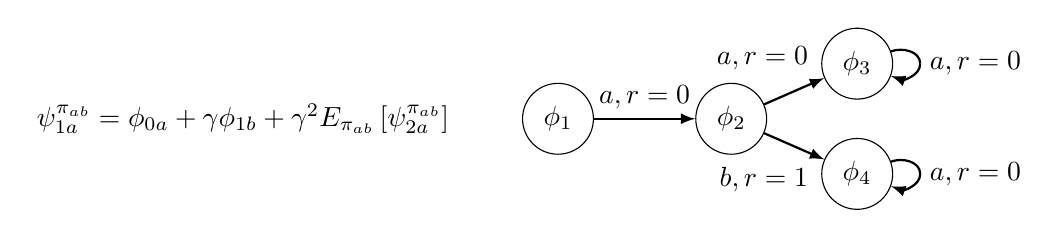
\begin{tikzpicture}[domain=-3:3]
\node[circle,draw=black,minimum size=.9cm](phi1) at (1,    0) {$\phi_1$};
\node[circle,draw=black,minimum size=.9cm](phi2) at (3.2, 0) {$\phi_2$};
\node[circle,draw=black,minimum size=.9cm](phi3) at (4.8, .7) {$\phi_3$};
\node[circle,draw=black,minimum size=.9cm](phi4) at (4.8,-.7) {$\phi_4$};

\draw[thick,-latex] (phi1) -- (phi2) node[pos=.5, above] {$a,r=0$};
\draw[thick,-latex] (phi2) -- (phi3) node[pos=.9, above left] {$a,r=0$};
\draw[thick,-latex] (phi2) -- (phi4) node[pos=.9, below left] {$b,r=1$};

\node[anchor=west](phi3out) at (5.6, .7) {$a, r=0$};
\path[] (phi3) edge[thick,out=20,in=90] (5.6,.7)
	   (5.6,.7) edge[-latex,thick,out=-90,in=-20] (phi3);
	   
\node[anchor=west](phi4out) at (5.6, -.7) {$a, r=0$};
\path[] (phi4) edge[thick,out=20,in=90] (5.6,-.7)
	   (5.6,-.7) edge[-latex,thick,out=-90,in=-20] (phi4);

\node[](sf) at (-3,    0) {$\pmb{\psi}_{1a}^{\pi_{ab}} = \pmb{\phi}_{0a} + \gamma \pmb{\phi}_{1b} + \gamma^2 \mathbb{E}_{\pi_{ab}} \left[ \pmb{\psi}_{2a}^{\pi_{ab}} \right]$};

\end{tikzpicture} 